\documentclass{scrartcl}
\usepackage[T1]{fontenc}
%\usepackage{SRM2}
\usepackage{graphicx}
\usepackage{url}
\usepackage{color}
\usepackage{longtable}
\title{The PAMalyzer (v 0.0.1)}
\author{Florian Meerheim + The AviaNZ Team \\ \url{florian.meerheim@htw-dresden.de}}
\date{September 2026}

%\usepackage[usenames, dvipsnames]{color}

%Revise with track changes
\usepackage{soul}
\usepackage[normalem]{ulem}
\usepackage{multirow}
\usepackage{booktabs}
\usepackage{amssymb}
\usepackage[colorlinks=true,citecolor=black,urlcolor=black,linkcolor=blue]{hyperref}

\begin{document}
\maketitle

WORK IN PROGRESS!

This is the user manual for $\blacktriangle$ version xxx of the PAMalyzer program.
The PAMalyzer is based on AviaNZ, a software for bioacoustic analysis (\url{http://www.avianz.net}).
There are so many changes compared to AviaNZ that I decided to name it differently.
The most obvious are (i) the ability to classify your recordings with the BirdNET classiers, and (ii) several features to ease the analysis of the BirdNET results with filtering and sorting options.
The purpose of this manual is to help you get started with using the PAMalyzer.
Furthermore a 'Cheat Sheet' is provided which you can find in the same directory as this manual or within the program under Help. 


\section*{Quick-Start}

\begin{enumerate}
	\item \textbf{Set operator}: On first startup PAMalyzer will ask you to enter an operator name for future reference. More information in \nameref{sec:GettingStarted}.
    \item \textbf{Open an audio file}: If you did not use PAMalyzer before an example file will be loaded. You can use the \textit{Open sound file} option in the \textit{File} menu or press \texttt{Ctrl+O}. See \nameref{sec:OpenFiles} for details.
    \item \textbf{Choose a database}: All annotations in PAMalyzer are stored in a database. The default database will be good for first tests. Choose another database via \textit{Annotations>Database>Choose database} if you start productive work (see the \nameref{sec:database} section for more information).
    \item \textbf{Classify recordings}: To classify your audio files launch BirdNET via \textit{Analysis>Classify recordings with BirdNET}. Find more detailed information in the \nameref{sec:BirdNET} section.
    \item \textbf{Review detections}: PAMalyzer offers plenty of options for purposefull reviewing and filtering of detections. See the \nameref{sec:review} section for a full workflow.
    \item \textbf{Export results}: Export annotations and summary Excel files via the \textit{Export} options in the \textit{Annotations} menu.  Refer to the nameref{sec:outputs} section for the export formats.
\end{enumerate}

\tableofcontents
\newpage
\section{Introduction}

The PAMalyzer enables you to: 
\begin{itemize}

	\item Show and navigate through spectrograms of audio files
	\item Manually label bird calls in audio files 
	\item Use the BirdNET classification models on your data 
	\item Review the results of the BirdNET classification process

\end{itemize}
We will walk you through them individually.
If you are using PAMalyzer the first time the section \nameref{sec:GettingStarted} is a good starting point. 


\section{Installation and Setup}

For Windows users there is a downloadable installation file available on the github page \url{https://github.com/FloMee/PAMalyzer/releases}.
This should work for most users.

If you plan on using the software under Linux or MacOs, follow the instructions in the ReadME to install the software from source.

On Windows some files will be placed in your home directory, which may be somewhere like \url{C:/Users/username/AppData/Roaming/PAMalyzer}. On Mac and Linux they will be in \url{~/.PAMalyzer}.


\section{Getting Started}
\label{sec:GettingStarted}

On the first startup the program will ask you to give a name for the operator.
This is useful to keep track of who has looked at different files.
After confirming the main interface (figure \ref{fig:Interface}) shows up.
By default a demo audio file is shown.
If you want to move to a new directory, either use the `..' option to navigate around your computer's file system, or use the \textit{Open sound file} in the \textit{File menu}. 

\begin{table}[ht!]
	\centering
	\begin{tabular}{p{0.9\textwidth}}
		\textit{\textbf{Note:} PAMalyzer can load audio files in wav format. Other audio files should be converted to wav format. PAMalyzer assumes that audio files are recordings in mono (single microphone) sound. If there are other channels, only the first one is loaded. Very long recordings can be used, but it is generally easier if they are split into shorter files.}
	\end{tabular}
\end{table}


\subsection{The Main Interface}


\begin{figure}[htpb]
	\centering
	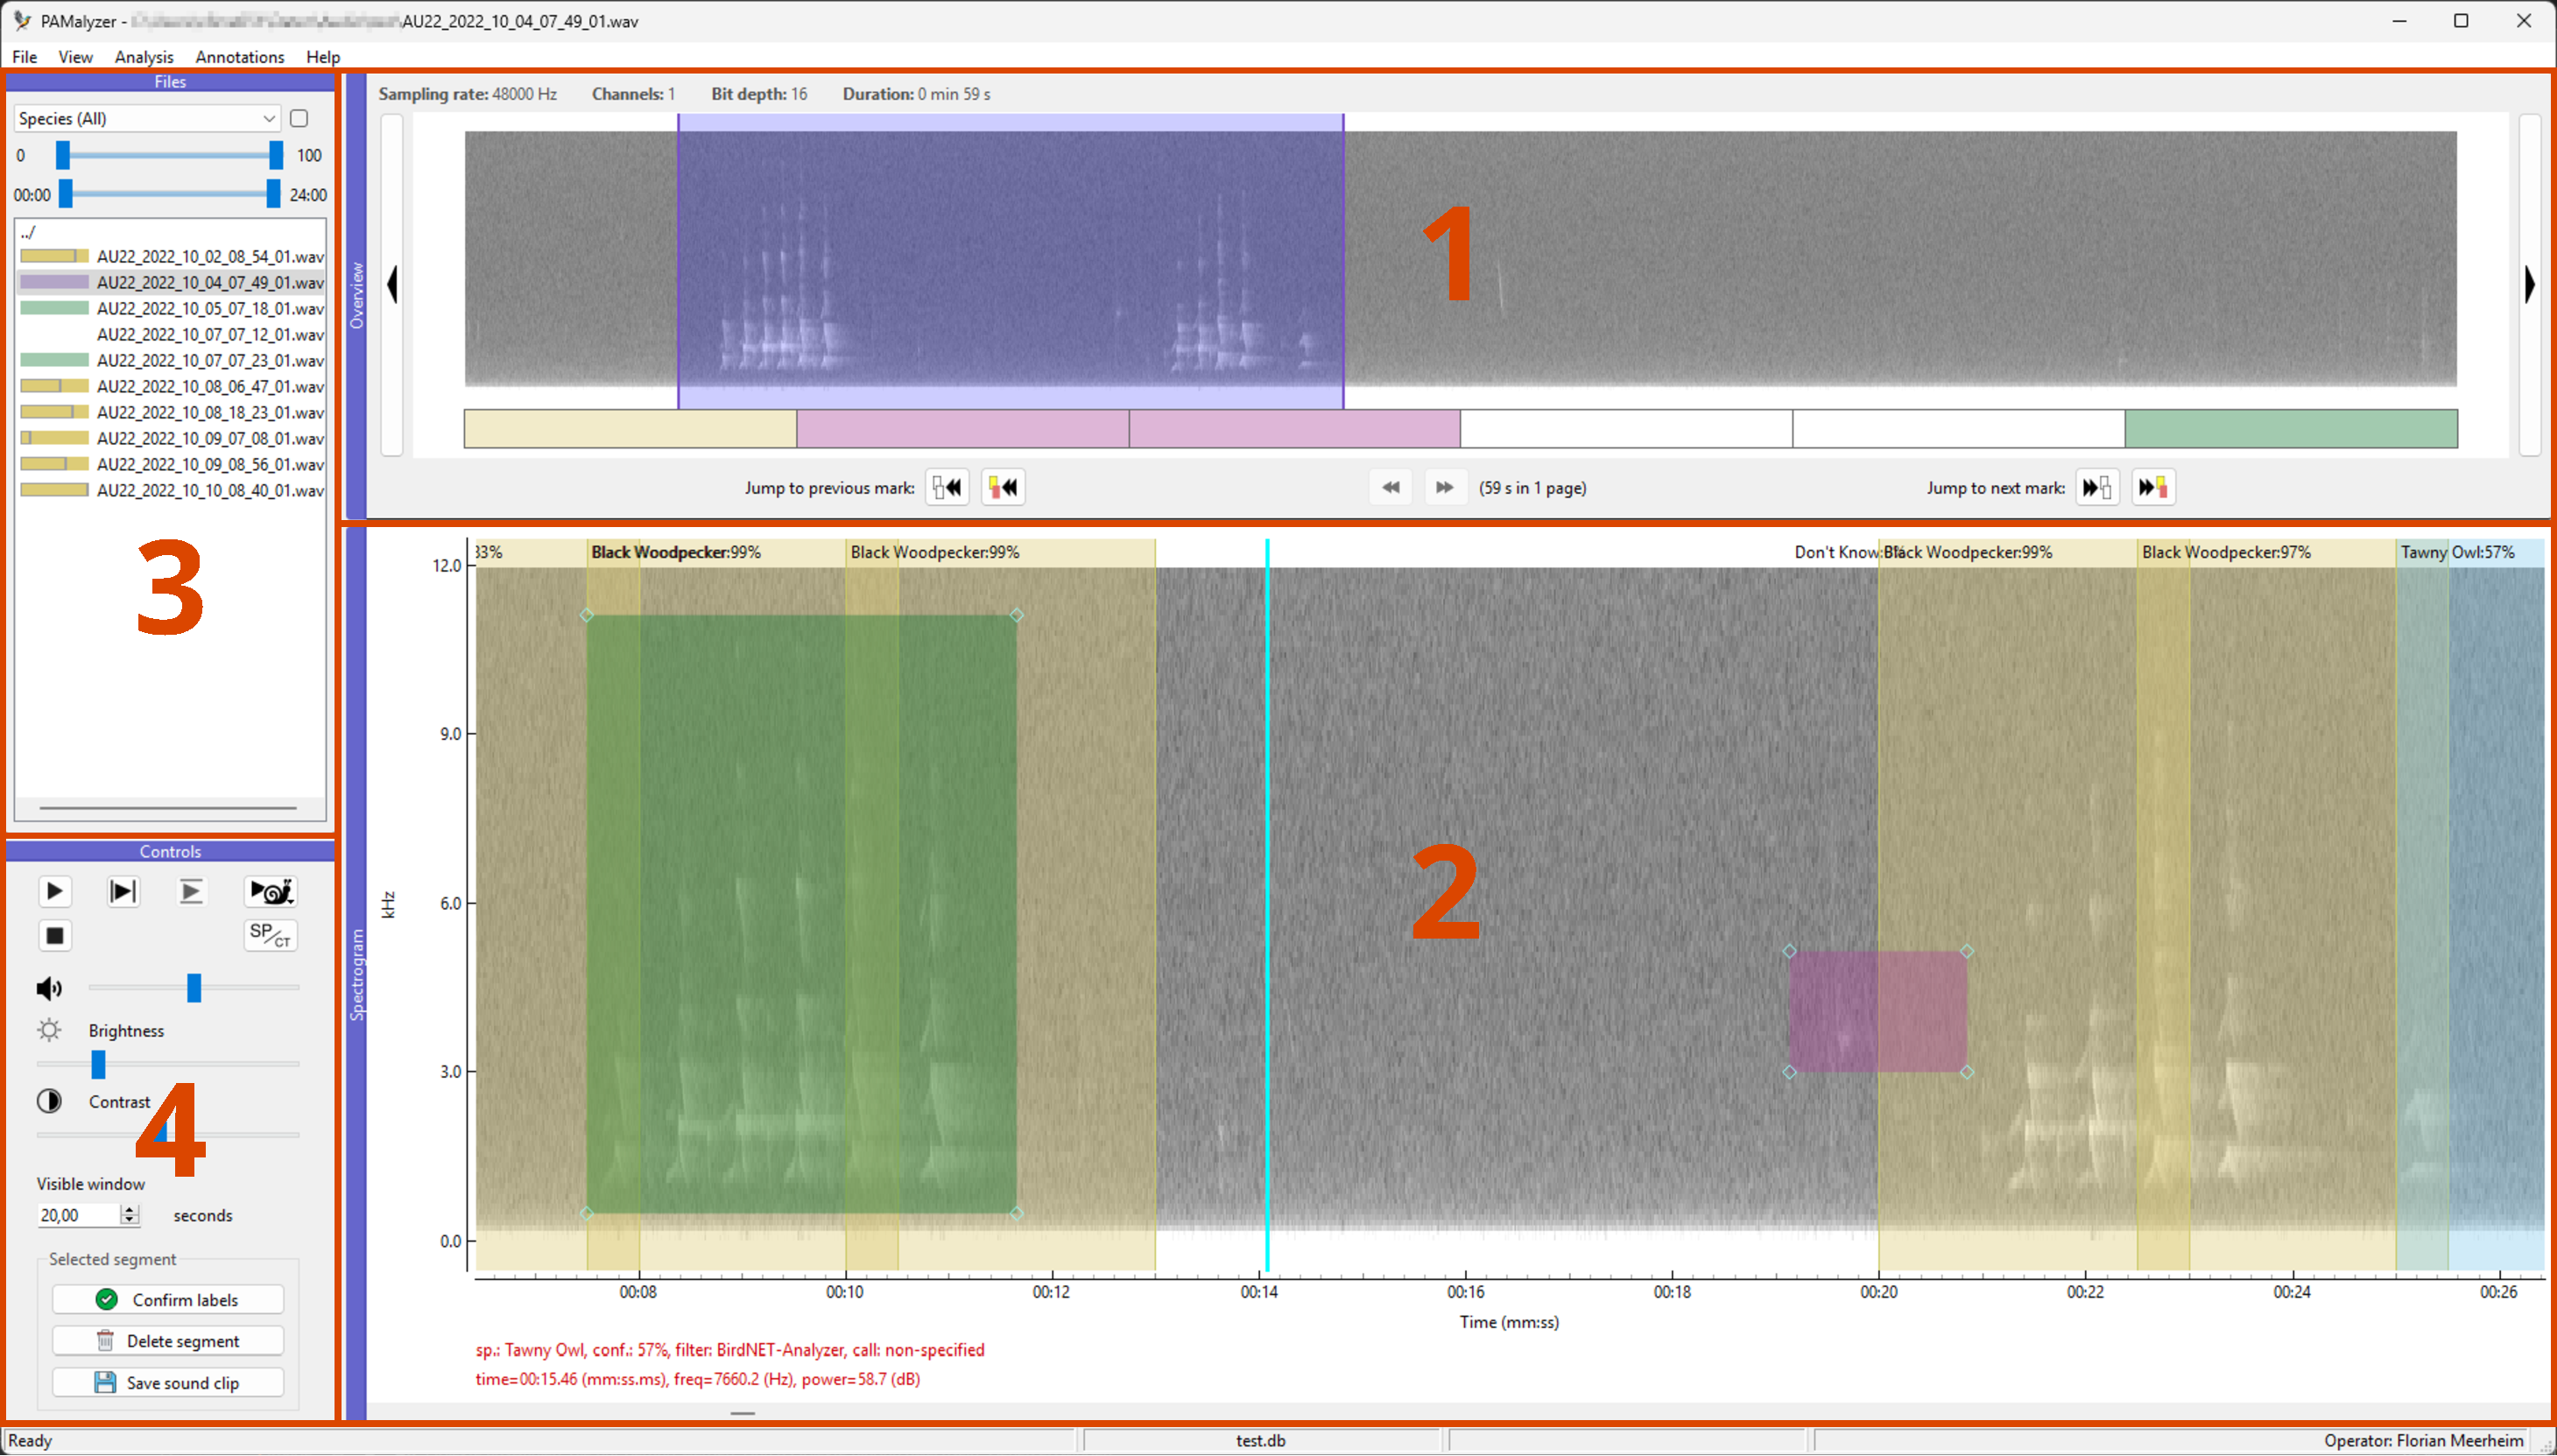
\includegraphics[width=.95\textwidth]{Figures/PAMalyzerInterface.pdf}
\caption{The interface of the \textit{Manual Processing} mode with its different components.}
	\label{fig:Interface}
\end{figure}


The name of the current file is shown in the title of the window (1). Below that there are four separate areas of the screen. Each has its name in a blue bar. They are:
\begin{description}
	\item[Overview (2--6)] This area shows a spectrogram of the first 5 minutes of the current audio file (labelled 2 in the figure).
		The blue section indicates the part you are looking at in the Spectrogram plot below.
		It can be moved by using \texttt{Left} and \texttt{Right} arrow keys, dragging the centre of the box, by clicking on the left and right arrow buttons ($\blacktriangleleft, \blacktriangleright$) next to the spectrogram (3) or by using the buttons in the bar below the spectrogram (4).
		It can be resized by dragging the ends of the box.
		Below the bar with buttons there are double arrow buttons ($\blacktriangleleft\blacktriangleleft, \blacktriangleright\blacktriangleright$, labelled 5 and 6).
		With the buttons labelled 5 you can open the next 5 minutes page of the audio file, provided it exists.
		The other buttons (6) you can use to jump with the blue section to the next annotation segment.
		%The double arrow buttons labeled 4 in the figure move to the previous or the next 5 minutes of the file (if they exist), while the ones labeled 6 move to the next annotation (see section <++> for details).
	\item[Spectrogram (7--9)] In this area the spectrogram of the blue section in the Overview area is shown.
		Here you can add and modify annotations.
		The axes for the image shows frequencies on the vertical axis and time on the horizontal axis (8).
		The time is true time if PAMalyzer can read that from the file, and starts from time 0:00 otherwise.
		There is also a scroll bar to move through the current page (9).
		The way in which you annotate recordings is described in the section \nameref{sec:ManualLabel}.
%		the current operator and reviewer are shown in 10.
	\item [Files (10--11)] This is the list of audio files (11) in your current directory.
		Use the \texttt{Up} or \texttt{Down} arrow buttons on your keyboard to navigate through the file list.
		You can also double-click on a file to select and open it.
		The file icons next to the file names indicate the status of the audio file. 
		This is described in detail in the section \nameref{sec:ColourCodes}.
		There are several filtering options (10) to reduce the file list. 
		These are described in \nameref{sec:FilterFileList}.
		%Files that have not been opened in PAMalyzer do not have an annotation to their left.
		%Otherwise, a small box is shown.
		%If the box is empty (white) then there are no segments of call annotated within it.
		%If the box is green, then there are, and they all have species annotation.
		%If the box is yellow then some are uncertain (either because the user added a question mark, or because an automated filter processed it and the output has not been confirmed).
		%It the box is red then there are segments labelled as 'Don't Know'. 

%The double arrow button on the top right of this area (labelled 10) moves on to the next file.


	\item[Controls (12--14)] The buttons in this area are referring to the Spectrogram area. 
		You can playback the audio file (12), modify the appearance of the plots (13) and process any segment that is currently selected (14).
		For more details, see \nameref{sec:play}.
	\end{description}

There is an optional fifth area, which is the Amplitude plot.
If you want to see it, select \textit{Show amplitude plot} in the \textit{View} menu.
Select the option again to hide it.
You can also hide the \textit{Files} and \textit{Overview} area in the same way.
PAMalyzer will remember your choice in future uses.

\begin{table}[ht!]
	\centering
	\begin{tabular}{p{0.9\textwidth}}
\textit{\textbf{Note:}
	You can drag the five screen areas around and reorder them if you wish, by dragging the blue bar on the top or left of them with the name of the section in it.
	You can also make them into their own windows by double-clicking on the blue bar.
If you decide that you made a mistake doing that, then there is an option in the \textit{Actions} menu to \textit{Put docks back} that returns them to the original configuration.}
	\end{tabular}
\end{table}

There are two other parts to the interface:
	\begin{description}
	\item[Menu] The menu at the top of the screen. 
	\item[Status Bar] At the very bottom of the screen there is an area that gives any status updates from the program (15), and on the right, information about the currently selected Reviewer and Operator (16).
	\end{description}



\subsection{Cheat Sheet}

You can find a Cheat Sheet with the most important navigation options, especially shortcuts in the \textit{Help} menu under \textit{Cheat Sheet}.
Especially in the review process after the classification of your audio files with BirdNET it can help a lot.


\section{Open Audio Files}\label{sec:OpenFiles}
\subsection{Spectrogram}\label{sec:spectrogram}


\begin{itemize}
	\item The main spectrogram plot (7) shows a section of the current audio file. The part you are looking at is highlighted in blue in the overview spectrogram (2).
	\item The axes of the spectrogram are time on the horizontal axis (8) and frequencies on the vertical axis.
	\item The times will be true times if file names contain the time stamp in the format \textit{\textless year\textgreater\textless month\textgreater\textless day\textgreater\_\textless hour\textgreater\textless minute\textgreater\textless second\textgreater}, or time from start of file otherwise. 
	\item Sometimes spectrograms don't look good initially, for example because of high noise.
		You can modify the brightness and contrast of the spectrogram using the two sliders in the Controls section (13). 
	\item You can also use a different colour scheme, and invert the colour map (swap black and white), by choosing the relevant options in the \textit{View} menu.
	\item To change the computation of the spectrogram you can use the \textit{Change spectrogram parameters} from the \textit{View} menu. The options are described in detail in section \ref{sec:spectrogram2}.
	\item It is possible to display information about where the mouse is pointing on the spectrogram (time, frequency, energy value) below the axis by choosing \textit{Show pointer details in spectrogram} from the \textit{View} menu, and to switch it off the same way.
\end{itemize}


\subsubsection{Changing the Spectrogram Computation}\label{sec:spectrogram2}

\begin{itemize}
	\item Selecting \textit{Change spectrogram parameters} from the \textit{View} menu will produce the following dialog box:

\begin{center}
    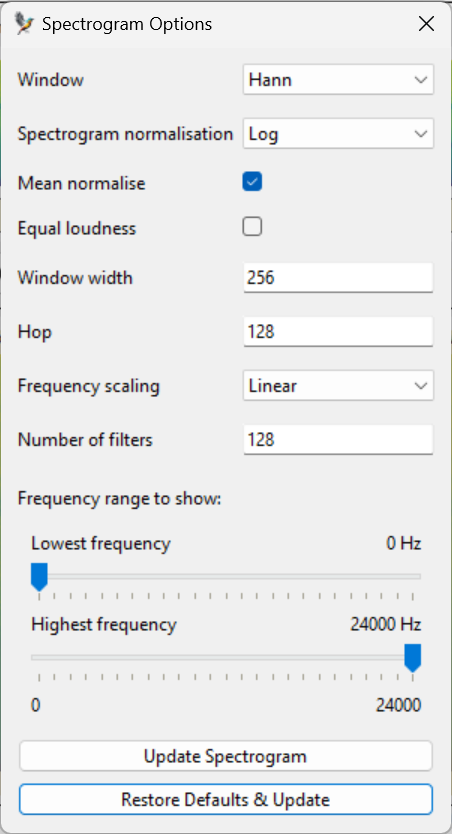
\includegraphics[width=.4\textwidth]{Figures/SpectrogramOptions}
\end{center}

\item You can change some of the parameters that are used to produce the spectrogram:

\begin{itemize}
\item The window function (default: Hann) controls how the spectrogram combines sounds across the time range. 
\item Mean normalisation and equal loudness try to make the spectrogram energies more even.
\item Multitapering uses multiple windows to make a better estimate of the spectrogram, but performs a lot of computation, and can therefore be slow.
%\item Spectrogram reassignment also tries to make a better estimate.
\item The window width and hop size control how much of the audio file makes up one spectrogram bin, and how they overlap. A big window size will improve frequency resolution, but reduce time resolution, and vice versa. The hop size controls how much the spectrogram time bins overlap. It is computationally more efficient if these numbers are powers of 2 (such as 256, 512, 1024).
\item The frequency range sliders let you change the visible frequency range in the main spectrogram window. This can be useful if you want to focus on only part of the range.
\end{itemize}

%\item If you want to know more about these options, look on the PAMalyzer webpage, in the `Technical Details' section. 
%\item You can also just try changing them and see if it makes your spectrograms clearer.
\end{itemize}


\subsubsection{Denoising}\label{sec:denoising}

\begin{itemize}
	\item When audio files are particularly noisy, it can be helpful to remove some of that noise. PAMalyzer currently provides three ways to do this (via the \textit{Denoise} option in the \textit{Actions} menu):
\begin{description}
\item[Wavelets] This is our main method, and tries to preserve the bird call perfectly. 
\item[Bandpass] Suppresses all frequencies outside a restricted range (which you specify) so that you can concentrate on the frequency range where calls that you are interested in can be seen.
\item[Butterworth bandpass] Another way to compute a restricted frequency range.
\end{description}
\item You can save the denoised audio files, and undo the denoising if it does not help.
\end{itemize}

\section{Navigation}
\paragraph{Navigate through Files}

To quickly navigate through the list of files and the files themselves it is highly recommended to use the arrow keys on the keyboard:
Use the \texttt{Up} and \texttt{Down} arrow keys to open the previous or next audio file in the file list.
Use the \texttt{Left} and \texttt{Right} arrow keys to move backward and forward through the audio file.

%\paragraph{Zooming and Scrolling}
But there are a lot of more options:
\begin{itemize}
	\item To open an audio file: 
	\begin{itemize}
		\item Use the \texttt{Up} or \texttt{Down} arrow keys to open the next or the previous file in the file list.
		\item Use \textit{Open audio file} in the \textit{File} menu if you want to open an audio file in another directory.
		\item Double Click on a file in the list of files.
		\item Double Click on a folder will open that folder; the `..' option at the top of the list takes you up one directory.
	\end{itemize}
	
	\begin{table}[ht!]
		\centering
		\begin{tabular}{p{0.9\textwidth}}
			\textit{\textbf{Note:} If some of the filter options in the Files area (10) are applied, some of the files might be hidden within the file list. In this case the \texttt{Up} and \texttt{Down} arrow keys apply only for the visible files. The shortcut \texttt{Alt + Up/Down} in contrast includes also the hidden files, so that you can still reach them.}\\
		\end{tabular}
	\end{table}

	\item To move within a file:
	\begin{itemize}
		\item Press the \texttt{Left} or \texttt{Right} arrow keys.
		\item Drag the blue highlight in the overview spectrogram. 
		\item Click on any of the boxes in the bar below the overview spectrogram.
		\item Click on the left or right arrows on the left and right of the overview spectrogram.
		\item Drag the scroll bar below the spectrogram.
	\end{itemize}
	\begin{table}[ht!]
		\centering
		\begin{tabular}{p{0.9\textwidth}}
			\textit{\textbf{Note:} According to the set page size (defaults to 5 minutes) in the \textit{\nameref{sec:interfacesettings}} long files are split into several pages. To open the next or previous page of an audio file use the double arrow buttons (5) below the overview spectrogram or the shortcut \texttt{Shift + Left/Right}. More details in: \nameref{sec:longfiles}.}\\
		\end{tabular}
	\end{table}

	\item To change the amount of the file that you can see (the visible width): 
	\begin{itemize}
		\item Drag the ends of the blue highlighted section in the overview spectrogram.
		\item Change the \textit{Visible window width (seconds)} in the Controls dock by clicking on the up and down arrows, or typing in a new number.
	\end{itemize}

	\item You can also view a restricted amount of the spectrogram by reducing the visible frequency band, see Section \nameref{sec:spectrogram2}. 
\end{itemize}

\paragraph{Moving Through Long Files}\label{sec:longfiles}


According to the set page size (defaults to 5 minutes) in the \textit{\nameref{sec:interfacesettings}} long files are split into several pages.

\begin{itemize}
	\item To move to the next or previous page: 
\begin{itemize}
	\item Use the double arrow buttons labelled (5) or
	\item press \texttt{Shift + Left/Right} arrow keys. 
\end{itemize}
	\item The program tells you which page you are currently on, and how many there are in total. 
	\item You can change the page size and the amount of page overlap by choosing the relevant options in the \textit{\nameref{sec:interfacesettings}} in the \textit{View} menu. 
	\item The times on the axis below the spectrogram show locations in the full file.
	\item Note that operations like denoising and segmentation (described in the section \nameref{sec:action}) apply to the visible 5 minute portion of the file, not the whole file.
\end{itemize}


\section{Annotate Recordings}\label{sec:ManualLabel}
\subsection{Overview}

The aim of the labelling process is to add further information to the audio file.
For this purpose PAMalyzer uses labeled segments.
A segment is a specific range in time and frequency within the spectrogram.
Together with the information about time and frequency a species label (e.g. a bird species) and a call type label (for specific call types of the species) can be stored.

\begin{itemize}
	\item To create segments, click and drag with the left mouse button on the Spectrogram.
		(The action of left and right mouse buttons can be swapped over in the \textit{Interface settings}.)
	\item To select segments, click on them with the right mouse button (pressing control on the keyboard when clicking on a Mac).
		The segment will turn blue when it is selected.
	\item If you find that the colours make it hard to see the data underneath the boxes you can make them transparent using the \textit{Make dragged boxes transparent} option under \textit{Annotation} in the \textit{\nameref{sec:interfacesettings}}.
		You can also choose different colours there if you have particular preferences.
	\item Segments are saved automatically, so that you can't lose your work.
\end{itemize}


\subsection{Create and Label Segments}\label{sec:labelSegments}


\begin{itemize}
	\item There are three ways to create a segment. You change which of them to use in the \textit{Mouse settings} of the \textit{\nameref{sec:interfacesettings}} in the \textit{View} menu:

	\begin{itemize}
		\item \textit{(default)} Drag a limited frequency band box (i.e., click and hold the mouse button and drag the mouse to the correct end point in both time and frequency).
		\item Start and stop a limited frequency band by clicking (i.e., click once at the correct time and frequency for the start of a segment, and then again at the time and frequency for the end).
		\item Start and stop a full frequency band by clicking (i.e., click once at the correct time for the start of a segment, move the mouse to the end, click again, the box covers all frequencies).
	\end{itemize}
	
	\item When you create a new segment, a drop-down menu will appear asking you to choose a label for that segment. 

	\begin{itemize}
		\item To choose the type of bird, click on the name. 
		\item If the species isn't in the list, move to `Other'. 
		\item If it isn't in the second list, at the bottom of that list is a selectable box (it probably says `Albatross'). Clicking on it provides the complete list of birds. 
		\item If there is something missing from there, choose Other' from it, which is at the very end. It will ask you to enter a name, as Genus (Species); e.g., `Kiwi (Little Spotted)'. 
		\item If there is only a single example of the genus, you can miss out the species, e.g., `Kakapo'. 
		\item The new name you add will then appear in the list. 
		\item If you click anywhere on the screen except on a bird name in the menu then the menu will disappear and the bird type will be labelled as `Don't Know'. 
		\item The bird list that we are using is based on the one that DOC use, and is meant to cover all the bird species that we know about in New Zealand. 
		\item You can add new species individually using `Other' in the menus.
	\end{itemize}
		\begin{table}[ht!]
		\centering
		\begin{tabular}{p{0.9\textwidth}}
			\textit{\textbf{Note:} The original version of PAMalyzer comes with a bird list for New Zealand. In the list the species names are given as 'Genus (Species)'; e.g. 'Kiwi (Little Spotted)'. Given it in that way a submenu for every genus is created with the species in it. Although this works great for common species names in English, it doesn't in other languages. It is possible to use other bird lists (that do not necessarily have to follow this formatting) using the \textit{\nameref{sec:interfacesettings}}.}\\
		\end{tabular}
	\end{table}


	\item By default the lists of bird names updates dynamically, so that bird types you have chosen appear at the top of the list.
		If you don't like that, then you can disable it in the \textit{\nameref{sec:interfacesettings}}. 
	\item When creating a segment, you can give it the same label as the previous segment by pressing the \texttt{Shift} key on the keyboard when you create the segment.
		The program will then give the segment the same label as the previous box that you labelled, without showing you the list.
		This is very useful when there is one bird calling repeatedly.
	\item You can also show that you are uncertain by pressing the \texttt{Ctrl} button when you click to segment (command button on a Mac computer).
		The names of the birds will then have a question mark after them.
	\item You can choose whether or not to allow more than one species per segment.
		This can be useful for recordings of the dawn chorus and where you just want to label presence of a set of species.
		Use the \textit{Default to multiple species} in the \textit{\nameref{sec:interfacesettings}} to allow this.
		Then, when you choose a bird from the list it will be ticked, and the menu will not close automatically, allowing you to make multiple selections.
		To unselect something, click on it again.
		When you make a new segment, `Don't Know' is selected by default.
		Choosing any other option deselects `Don't Know'.
		You can reselect it if you do want that label as well. 
	\item PAMalyzer also allows you to specify a call type.
		This could be the difference between male and female vocalisations for e.g., kiwi, or different calls types such as `more-pork' or `cree' for ruru.
		You can add specific call types manually.
		To swap between seeing the species and seeing the call type label use the SP/CT button (\includegraphics[scale=0.5]{Figures/SPCT}) on the right of area 12 of the Controls panel or press the \texttt{Tab} key.

\end{itemize}


\subsection{Update Segments}
\begin{itemize}
	\item If you select a segment that already exists by clicking on it then it will turn blue.
		Click on it again and the menu will reappear so that you can correct mistakes.
		This will be either the species label or the call type label depending on the SP/CT button.
	\item Segments have blue diamonds at the corners, so that you can resize them, or you can move the whole segment by dragging it (this works even when it isn't selected). 
	\item Segments can be deleted by selecting them (so that they turn blue) and then clicking on the \textit{Delete Current Segment} in the Controls or pressing the \texttt{Delete} or \texttt{Backspace} key on the keyboard. 
	\item To delete all of the segments from the current file, use the \textit{Delete all segments} option in the \textit{Actions} menu or the shortcut \texttt{Ctrl + D}. 
	\item You can disable the making and updating of segments (to avoid making segments by mistake) by selecting \textit{Make read only} from the \textit{View} menu.
\end{itemize}


\subsection{Coulour Codes}\label{sec:ColourCodes}

\begin{itemize}

\item The segments that are drawn on the screen have different colours. These colours are changeable in the \textit{Interface settings}, but by default are:
	\begin{description} 
	\item[Blue] This segment is currently selected. You can play it by pressing the buttons in the Controls area (see Section~\ref{sec:play}), or give it a new label by clicking on it again, or delete it. 
	\item[Green] This segment has been labelled with a bird name and a confidence value of 100. These are either manually created segments or the manually confirmed results of an automatic filter.
	\item[Yellow] This segment has been labelled with a bird name and a confidence value between 0 and 100. These are either manually created segments with a question mark (by pressing \texttt{Ctrl} while dragging the box), or the row result of an automatic filter. 
	\item[Red] This segment has been labelled as `Don't Know'. Its confidence value is 0.
	\end{description}

\item These colours match the rectangles underneath the Overview:

\begin{center}
\includegraphics[width=.9\textwidth]{Figures/Overview}
\end{center}

\item For each 10 second segment of the file, these boxes are:
	\begin{description} 
 	\item[White] if there are no segments, or
	\item[Red] if there are `Don't know' segments, or
	\item[Yellow] if there are questionable segments, or 
	\item[Green] if all the segments in that section are labelled with definite species. 
	\end{description}
	
\item You can click on those boxes, and they will update the main spectrogram plot to show that section of the file. This is a useful way to move through the file quickly.
\item The described color scheme also matches the colors of the file icon in the file list. 
	\begin{description}
		\item[White]  if there are no segments in the file or directory, or
		\item[Red] if there are 'Don't know' segments, or
		\item[Yellow] if there are questionable segments, or
		\item[Green] if all the segments in the file or directory are labelled with definite species.
	\end{description}
	\item Moreover, the grey box in the file icon indicates the maximum confidence value found in the segments of the file.
	\begin{table}[ht!]
		\centering
		\begin{tabular}{p{0.9\textwidth}}
			\textit{\textbf{Note:} The filtering options for the file list (10) also effect the file icon. If the segments in the file do not match the set conditions the file icons turn white. You can use this feature to quickly search for candidate recording after the classification process with BirdNET. The workflow with BirdNET is described in the section \nameref{sec:BirdNET}}\\
		\end{tabular}
	\end{table}
\end{itemize}


\section{Classify Recordings with BirdNET}

\label{sec:BirdNET}
An overview of the workflow with BirdNET is shown on figure \ref{fig:workflow}.
It is divided into several steps, beginning with the classification process of the audio files, continuing with  the filtering and reviewing of the detections coming to the summary of the results.

\begin{figure}[htpb]
	\centering
	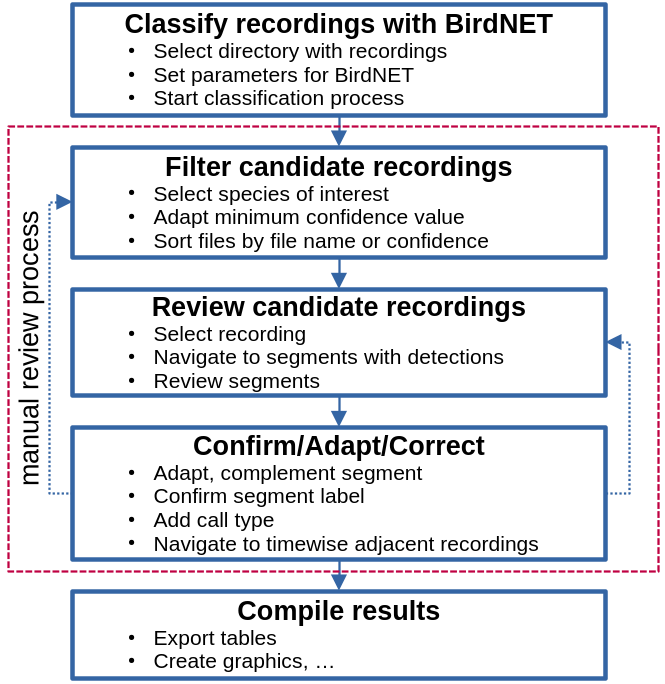
\includegraphics[width=0.65\textwidth]{Figures/BirdNET_Workflow.png}
	\caption{Overview on the classification and review process using the BirdNET classifiers.}
	\label{fig:workflow}
\end{figure}



To start the analysis of your audio files with BirdNET you first have to specify different parameters.
You can reach the input form by clicking on \textit{Recognisers $\rightarrow$ Classify recordings with BirdNET} in the menu.
\begin{center}
	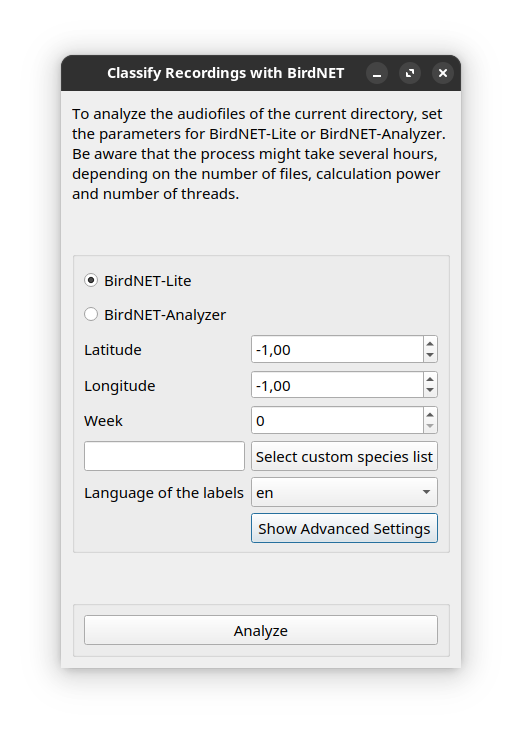
\includegraphics[width=.5\textwidth]{Figures/BirdNET_Settings}
\end{center}

In this window the parameters for BirdNET-Lite or BirdNET-Analyzer can be set.
The button \textit{Show advanced settings} gives even more options.
The meaning of the different parameters is explained in the cheat sheet that you can find over \textit{Help $\rightarrow$ Cheat Sheet}.

If you are using BirdNET for the first time it is recommended to just set the geographical location with specifying \textit{Latitude} and \textit{Longitude} and provide the time of the year with the week parameter.
The other parameters can stay with default values.

After the parameters are chosen, the analysis can be started by clicking on the \textit{Analyze} button.
That will classify all the recordings in the current directory including subdirectories.
With that it is possible to, for example analyse all the recordings of different locations within one recording session.
If you specifically want to use this possibility you can change to an upper directory via the '../' in the file list.

Depending on the number of recordings to classify, the CPU power and the number of threads the classification process might take minutes or several hours.
Keep that in mind while choosing your parameters. 
It might also be helpful to test your desired settings on a small test dataset to see if proper results are obtained.


\section{Review Classifier Detections}\label{sec:review}
\subsection{The output of BirdNET}
Before the actual workflow is described the output of BirdNET will be introduced. 

Internally BirdNET cuts your recordings into chunks of 3 seconds that overlap more or less depending on the set overlap parameter.
For each of these chunks BirdNET produces a list of all classes BirdNET can distinguish (mainly bird species, hereafter species).
To each of these species a confidence score ranging from 0 to 1 is attached.
With setting the different parameters of BirdNET (for example: minimum confidence, latitude, longitude, week, custom species list) this list is reduced to a minimum of at most a few species. 

For interpreting the results it is important to understand that the confidence scores are not calibrated. That leads to two important things:
\begin{itemize}
	\item The confidence score is not a true probability or certainty value. A value of 0.8 does not mean, that on average the species can be found in 8 out of 10 segments labelled with this certainty value.
	\item The confidence scores can not be compared across different species. A value of 0.8 can have a completely different meaning for a pygmy owl than for a capercaillie.
\end{itemize}


\subsection{Sorting the List of Files}

By default the list of files is sorted by their file names. 
Usually the recordings include a timestamp in the format Year-Month-Date-Hour-Minute-Second - or similar. 
Sorting the files by file name means sorting by time in these cases as well.
In this mode moving to previous/following recordings in the file list also means moving to timewise adjacent recordings.

You can change the sorting behaviour of the list of files by using the option \textit{Sort files by maximum confidence} in the menu under \textit{View}.
This sorts the list of files descending by the highest confidence scores detected in the recording for the selected species. 
Moving to timewise adjacent recordings does not work in this mode anymore.


\subsection{Filtering Audio Files}\label{sec:FilterFileList}
After the classification process finished you will see that the file icons changed.
As described in the section \nameref{sec:ColourCodes} the color indicates different states of the segments in the file.
Moreover, the grey frame within the icon marks the maximum confidence score detected in the file.

The file icon always refers to the currently selected species. 
This can be selected after the classification process from the dropdown menu on top of the file list. 
The values after the species in this list indicate the maximum confidence score found for that species in the audio files of the current directory.
If you also tick the box next to that dropdown menu, the file list will reduce to the files in which the selected species are found. 

You can further reduce the list of files with changing the value of the slider below the dropdown menu.
With that it is possible to exclude all the audio files with a maximum confidence value for the selected species below the selected value.

Use these options to systematically search for audio files with high confidence scores for the specified species (considered ``candidate recordings'').

\subsection{Manual Review}

If a first audio file from the file list is selected you can jump to the first segment labeled with the selected species either with pressing the button \textit{Jump to next mark} below the overview spectrogram or by using the shortcut \texttt{Ctrl + Right}.

Use the play buttons to start the playback of the file.
Alternatively you can use the shortcut \texttt{Space} or \texttt{Ctrl + Space} to playback the visible area in the spectrogram or just the selected segment respectively.

The goal of this step is to review all the segments within the file for the selected species.


\subsection{Confirm/Change/Correct segments}

If the segment is checked it should be confirmed, changed or corrected right after it.
Only this way you can avoid to check the same segments and audio files again and again.

For that purpose different options exist:
\begin{itemize}
	\item To confirm the label of a selected segment use the \textit{Confirm labels} button in the \textit{Controls} area or simply hit the \texttt{Enter} key.
	\item Use your mouse to drag single segments to change their position.
	\item Use your mouse and the diamonds in the corners of a selected segment to resize it.
	\item Use the \textit{Delete segment} button or the \texttt{Delete} key to delete segments
	\item Use the \textit{Delete all segment} option from the \textit{Actions} menu or the shortcut \texttt{Ctrl + D} to delete every segment in the current file. 
		This can be handy if you want to replace a lot of BirdNET detections in a file with just one segment.
	\begin{table}[ht!]
		\centering
		\begin{tabular}{p{0.9\textwidth}}
			\textit{\textbf{Note:} If there are several species attached to a single segment you can only confirm all the labels. In that case confirm all the labels first and deselect the ``wrong'' species by simply clicking with the right mouse button on the segment and deselecting the species from the opening menu.}\\
		\end{tabular}
	\end{table}
\item If you can neither confirm nor refuse the label BirdNET has given to the segment it might be helpful to assign a custom `species' label. Later, this label can be used to filter out recordings with these doubtful segments. The process how you can add custom labels is described in \nameref{sec:labelSegments}.
	\item Additionally to the species label PAMalyzer provides the options to assign call type labels. 
		You can change the type of the labels that are shown in the segments by pressing the \textit{SP/CT} button in the controls area or with the \texttt{Tab} key.
		With right clicking on a selected segment a menu opens where you can select call types from a list or add a new call type for the specific species by choosing the \textit{Add calltype} option.
\end{itemize}

After that process you can go on to the next file using the \texttt{Down} arrow key.


\subsection{Include temporal adjacent recordings}

If a species was confirmed in an audio file it might be a good idea to look for further calls of the same species in the files that were recorded right before or after that.
Because of the filtering process it might be that these recordings do not appear in the file list anymore. 
Nevertheless you can reach those recordings by pressing the \texttt{Alt} key together with the \texttt{Up} or \texttt{Down} keys when moving on to the previous or next audio file.
For this option you have to sort the files by name, not by confidence score! 

This process might be helpful to gain further ecologically interesting information about the species.
Especially faint calls are still a challenge for recognizers like BirdNET.


\section{Database}\label{sec:database}
\subsection{Choose Database}
\subsection{Update file paths}
\subsection{Database design overview}
\section{The BirdNET Workflow}
\subsection{Summarise results}
If every candidate recording is reviewed the annotations can be exported to an Excel workbook.
For that you can use the \textit{Export all segments to excel} option from the \textit{Actions} menu.

This option creates several Excel files in the current directory.
The \textit{DetectionSummary\_Any\_sound.xlsx} contains every segment of all the species within the current directory including subdirectories. 
Furthermore, individual files for every species are created with the pattern \textit{DetectionSummary\_SpeciesName.xlsx}.

In these output files you can find a table in which for every segment the file, the start and end time of the segment as well as the minimum and maximum frequency and call type label are given.
In the Excel file for 'any sound' a further column with the species label is attached.

You can use these exported data for example for further analysis or simply to create graphics.

\section{Outputs}\label{sec:outputs}

The PAMalyzer program aims to provide detailed and easy-to-review outputs. An Excel file (with the name `DetectionSummary' followed by the species selected) will be generated with three sheets of outputs in the same directory as the files. If this file already exists, the new results will be appended to the end of each sheet. 

The three sheets of the Excel workbook are:
\begin{enumerate}
\item start and end times of each birdcall detected
\item presence/absence of the target species (or set of species) in each recording
\item  presence/absence of the target species (or set of species) in each time interval that the user specifies (by default 60 seconds)
\end{enumerate}

In addition to the Excel file, for each audio file PAMalyzer generates an annotation file of the automated detections that  the user can open and review in either the main interface or using the \textit{Review Batch Results} option. 


\section{Reference}
\subsection{Interface panels}
\subsubsection{Overview}
\subsubsection{Spectrogram}
\subsubsection{Files}
\subsubsection{Controls}\label{sec:play}


\begin{center}
\includegraphics[width=.25\textwidth]{Figures/Controls.png}
\end{center}

\begin{itemize}
	\item The buttons at the top of the controls block allow you to play the sounds. 

\begin{itemize}
	\item The top-left button is a normal \textit{Play} button. The button turns into a \textit{Pause} button while playing. Instead of the buttons you can start and pause the playback using the shortcut \texttt{Space}.
	\item While the sound is playing, the light blue bar in the spectrogram plot shows where the playback is up to. 
	\item When the sound is paused, you can drag this bar if you want to hear a particular part of the file. Move the mouse over it, and the bar will go red. Then click and drag (using the mouse button that does not make segments, by default the right button) to move it. 
	\item To stop playback and have the slider return to the start of the visible section, press the \textit{Stop} button.
	\item When a segment is selected (so that it is blue) you can use the three play buttons to the right of the stop button to play just that small segment. 
	\item The difference between these is:
	    \begin{itemize} 
		    \item the one on the left (\includegraphics[scale=0.3]{Figures/playsegment}) plays all the frequencies in the audio file (shortcut: \texttt{Ctrl + Space})
		    \item the one in the middle (\includegraphics[scale=0.3]{Figures/playBandLimited}) plays only the frequencies highlighted, so that you can isolate particular frequencies of a call. This is particularly helpful when there is high level of background noise in a particular frequency range, such as cicadas, or where there are overlapping calls in different frequency bands.
		    \item the one on the right (with the snail: \includegraphics[scale=0.03]{Figures/playSlow-w}) lets you play the segment at different speeds. Hold the button down to change it to 2x (twice as fast) or 1/2 or 1/4 speed. Note that the pitch also changes, but it can be interesting or useful to hear all the components of a call.
	    \end{itemize}
	\item You can change the volume of playback using the slider below the buttons. 
	\item The SP/CT button changes whether you control species labels or call type labels of the segments (shortcut: \texttt{Tab}).
	%\item The button that shows a brush denoises a segment to try and make it easier to hear the bird call.
\end{itemize}

\item The \textit{Brightness} and \textit{Contrast} sliders change the appearance of the spectrograms (2, 7), helping to see more sounds. 
\item The size of the \textit{Visible window} controls how much of the overview spectrogram (2) appears in the main spectrogram (7).
\item The \textit{Confirm labels} button makes a segment label certain. This is useful to confirm labels that were made by an automatic recogniser, or that the user was previously unsure about.
\item The \textit{Delete segment} button removes any segment that is selected (blue colour). 
\item The \textit{Save sound clip} button saves a selected segment as a short audio file.
\end{itemize}


\subsection{Interface settings}\label{sec:interfacesettings}

\begin{itemize}
	\item There are quite a few user-selectable options in PAMalyzer, which you can choose using the \textit{Interface settings} menu option in the \textit{View} menu, which will produce the following dialog box:
\begin{center}
    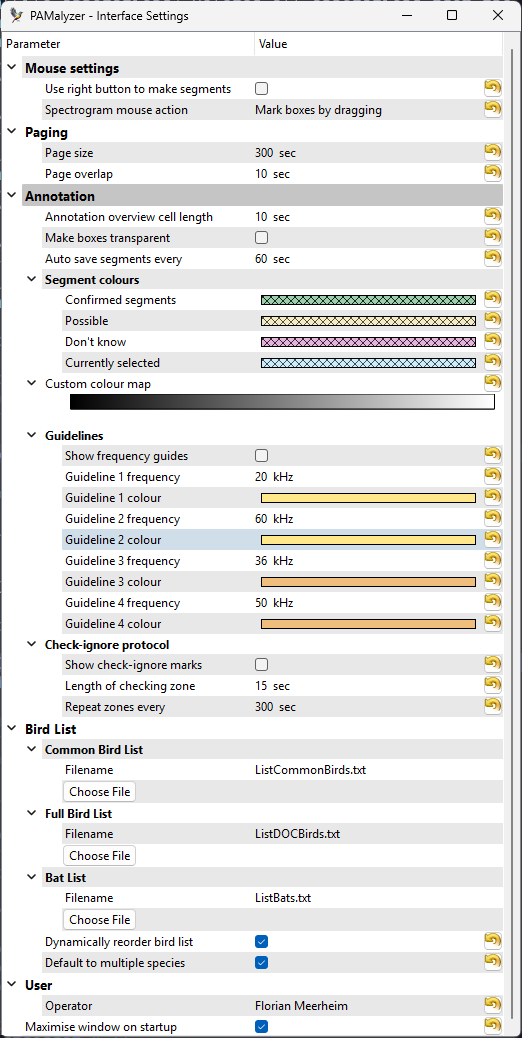
\includegraphics[width=.65\textwidth]{Figures/InterfaceSettings}
\end{center}

\item These options include:
\begin{description}
	\item[Mouse settings] Swap which mouse button selects segments and which creates them, and change the method of creating segments (described in detail in \nameref{sec:labelSegments}).
\item[Paging] The page is the length of spectrogram loaded into PAMalyzer at one time. By default it is 300 seconds (5 minutes). Note that longer times will require more memory and processing time. The amount of overlap between the pages can also be specified. The aim of the overlap is to make sure that calls aren't missed, and that segments are labelled accurately, at the page limits. 
\item[Annotation] 
\begin{itemize}
\item The first option in this section changes the length of the boxes in the Overview. 
\item The next enables you to make the labelling boxes transparent (so that only the outline of the box is shown) if you find it hard to see what is in a segment. 
\item By default, PAMalyzer save the segments you have made every 60 seconds. This can be changed, for example if you want to do it more often for safety. 
\item You can also change the colours of segments.
\item PAMalyzer has a check-ignore protocol for people who only annotate subsets of recordings. This puts a mark on the spectrogram in places where the user should be annotating the spectrogram, which you can control with these options.
\end{itemize}
\item[Bird list] There are two bird lists in PAMalyzer: the short list of common birds, and a longer list of all possibilities, together with a bat list. You can change these files for others (for example, to include non-New Zealand species). %See Section~\ref{sec:birdlists} for more information. 

You can also change the default behaviours of dynamically updating the list of common birds, and enable multiple species to be selected for a single segment. This can be useful for labelling things like the dawn chorus, but these segments will not provide good training data for new recognisers. 
%\item[Human classify] By default, PAMalyzer saves corrections that are made using the review options (see Section~\ref{sec:review}). 
\item[User] Enables you to set the operator and reviewer; this facility can also be found in the \textit{File} menu. You can also change whether or not the PAMalyzer window starts at full screen size, and whether or not the noise data must be completed for all files. 
\end{description}
\end{itemize}


\subsection{Menu options}
Most of the options for PAMalyzer are found through the menus. 
There are keyboard shortcuts for many of the menu items, which can be seen in the menus themselves.
You can find a reference of shortcuts in the section \nameref{sec:RefShortcuts}
\subsubsection{File Menu}
\begin{center}
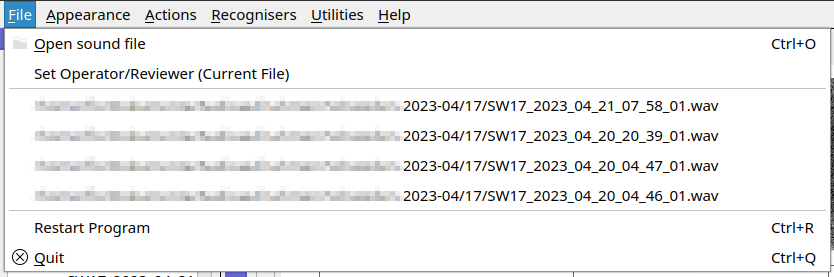
\includegraphics[width=.8\textwidth]{Figures/FileMenu}
\end{center}

\begin{description}
	\item[\textit{Open sound file}] Produces a file dialog so that you can choose a new audio file to open.
	\item[\textit{Set operator (Current File)}] Enables you to change the operator or reviewer that were specified when you started PAMalyzer. The change only applies to this file. 
	\item[List of recently used files] Makes it easy to revisit recent files.
	\item[\textit{Quit}] Does what it says.
\end{description}


\subsubsection{View Menu}

\begin{center}
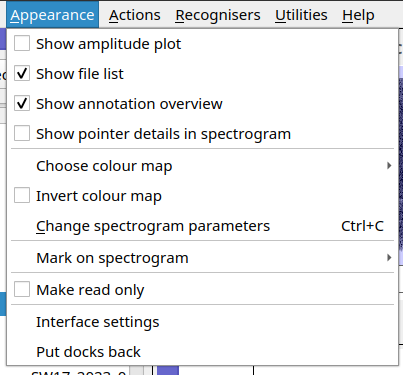
\includegraphics[width=.5\textwidth]{Figures/AppearanceMenu}
\end{center}

\begin{description}
\item [Changing appearance] The first four options in the menu hide or reveal the amplitude plot, file list, annotation overview, and information about where the mouse is pointing in the spectrogram. The ones that are selected are marked with a tick. 
\item [\textit{Choose colour map}] This enables the user to select a colour map for the spectrograms they prefer to the default grey one. To adjust the settings for the custom colour map, use the option \textit{Interface settings} on the bottom of the menu.
\item [\textit{Invert colour map}] By default, areas of high energy (frequencies where there is a call or other sound) are shown as the lightest colour, and low energy as dark. This can be swapped over with this option. Note that you will need to change the brightness and contrast using the \nameref{sec:play} area after inverting the colour map.
%\item [Make frequency axis tight] After bandpass filtering, this updates the spectrogram plot to stop showing the empty bands.
\item [\textit{Change spectrogram parameters}] A set of options to modify the spectrogram.  See the section \nameref{sec:spectrogram2} for more details. %Enables changes of the windowing function, width and increment of the FFT, and the option to not subtract off the mean. The `Multitapering' option can make very noisy spectrograms look better, but it takes a lot of computer time. 
%The two sliders at the bottom of the dialog enable the user to non-destructively show a limited frequency band in the spectrogram. The axis in the plot shows the range that is visible. 
\item [\textit{Mark on spectrogram}] There are some features that will help you spot bird calls or recognise them. We currently offer two options here: the fundamental frequency and points of high energy. To select one, choose it from the menu; select it again to remove it. They can help to find particular types of call. 
\item [\textit{Make read only}] When reviewing a segmentation it is possible to click on the plots by mistake, adding further segments. This option avoids this problem. It can be turned off by selecting it again. When read only mode is on, the message section at the bottom of the screen says so. 
\item[\textit{Sort files by maximum confidence}] This option sorts the list of files by the maximum confidence value of detections for the species selected in the \textit{Files} section. To enable a rank-based review process it excludes confirmed segments from sorting.

\item [Export view] Either export the overview spectrogram (from the overview panel) or the detailed spectrogram (from the spectrogram panel, including annotations) as image.
\item [\textit{Restore default layout}] Returns the various screen components to their original layout if they have been moved around. 
\item [\textit{Interface settings}] This option produces a dialog that enables the user to customise several things about PAMalyzer. See the section \nameref{sec:interfacesettings} for more details.
\end{description}


\subsubsection{Analysis Menu}\label{sec:action}

\begin{center}
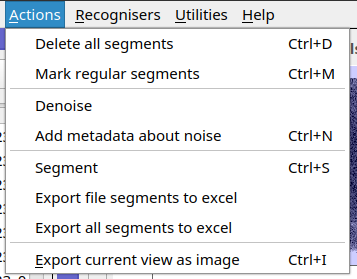
\includegraphics[width=.4\textwidth]{Figures/ActionsMenu}
\end{center}

\begin{center}
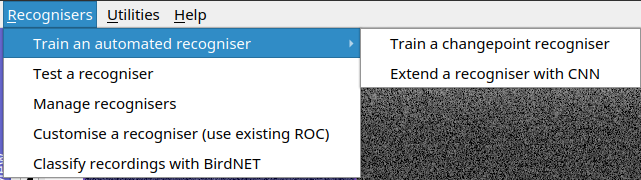
\includegraphics[width=.7\textwidth]{Figures/RecognisersMenu}
\end{center}

These options will mostly provide dialog boxes that ask you to make choices. 

\begin{description}
\item[Classify recordings with BirdNET] Choosing this option a window will open where you can set the parameters for BirdNET to classify all your recordings in the current directory and in all subdirectories. It is described in more detail in the section \nameref{sec:BirdNET}

\item [Denoise] Runs some programs that try to get rid of the noise in the audio file so that the birdcalls are easier to see. %You can also denoise a single segment by selecting it, and then pressing the button with a paint brush on in the `Controls' section (14). 
See section \nameref{sec:denoising} for more information.
% \item [Add metadata about noise] Allows the user to specify if the audio file is particularly corrupted by noise, and also to identify the type(s) if known. This can be an optional data field, or made compulsory for each file by choosing the appropriate option in the \textit{Interface settings}.
\end{description}



\subsubsection{Annotations Menu}

\begin{description}
	\item[Import Annotations]
	% \item [From Excel] If you have made user annotations in other programs that you want to import, this option will help to do it. Normally you can export annotations in csv or excel format, and then load them into PAMalyzer using this option.
	\item [From AviaNZ (.data files)] If you have made user annotations in other programs that you want to import, this option will help to do it.
	\item [From Raven (selection tables)] If you have made user annotations in other programs that you want to import, this option will help to do it.
	\item[Export Annotations]
	\item [To Excel (File)] This enables the user to save a summary of the annotation of the currently opened file into an Excel workbook (in the same location as the current audio file), as is described in section \nameref{sec:outputs}. 
	\item[To Excel (Directory)] This option summarises all the annotations of the current directory (including subdirectories) into Excel workbooks as described in section \nameref{sec:outputs}.
	\item[To database] If you want to copy a set of user annotations (for example to have them backed up, or to transfer them to another computer) without the wav files, but with the directory structure preserved, this option will do that. 
	\item[To .data files]
	\item[Export Audio]
	\item[Delete Annotations]
	\item[File annotations] Deletes all annotations from the currently open file
	\item[Directory annotations] Deletes all annotations in the currently open directory
	\item [Mark regular segments] Some users find it helpful to have an automatically generated segment box at regular intervals, for example to label all the birds in that segment under some statistical protocol. By default these are boxes are made to be 15 seconds long, with one box every 300 seconds (5 minutes) through the file. These options can be changed using the \textit{Check-Ignore protocol} area in the \textit{Interface settings}. There is also an option there to simply mark those areas rather than putting a segment box in place.
	\item[Database]

\end{description}

\begin{center}
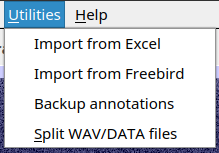
\includegraphics[width=.3\textwidth]{Figures/UtilitiesMenu}
\end{center}

\begin{description}
\item[Split WAV/DATA files] DOC AR4 recorders produce 15 minute audio files, but many other recorders produce far longer recordings. This can mean that you spend a lot of time going forward and backward through spectrogram pages. This option lets you split the audio files into shorter pieces. If you have already processed them, so that they have segments included, there will also be transferred to the new audio files.
\end{description}


\subsubsection{Help Menu}
\begin{description}
\item [Help] Gives access to this manual.
\item [Cheat sheet] Gives access to a cheat sheet with useful shortcuts and some information about the BirdNET classifier parameters.
\item[About] Shows you basic information about PAMalyzer.
\end{description}

\subsection{Menu items}

% \begin{longtable}{p{0.5\textwidth}p{0.45\textwidth}}
% 	\toprule
% \textbf{Menu Item} & \textbf{Function} \\
% \midrule
% \textbf{File Menu} & \\
% Open sound file & Opens a new audio file \\
% Set operator (Current File) & Changes the operator for the current file \\
% % List of recently used files & Lists recently opened files \\
% Quit & Quits the program \\
% \midrule
% \textbf{View Menu} & \\
% % Changing appearance & Hides or reveals the amplitude plot, file list, annotation overview, and information about where the mouse is pointing in the spectrogram \\
% Choose colour map & Set the color map for the spectrograms \\
% Invert colour map & Invert the color map chosen --> low energy as light and high energy as dark \\
% Change spectrogram parameters & Set spectrogram computation paramters: including window function, window width, and increment of the FFT \\
% Mark on spectrogram & \\
% — Fundamental frequency & Highlights fundamental frequencies in the spectrogram \\
% — Maximum energies & Highlists maxmimun energies in the spectrogram\\
% Make read only & Prevent addition of new segments annotations \\
% Sort files by maximum confidence & Sorts the list of files by the maximum confidence value of detections for the selected species \\
% Export view & \\
% — Overview spectrogram as image & Export the spectrogram of the whole file as image \\
% — Current spectrogram as image & Export the detail spectrogram as image - including annotations \\
% Restore default layout & Restores the original layout of the screen components \\
% Interface settings & Customize various settings in PAMalyzer \\
% \midrule
% \textbf{Analysis Menu} & \\
% Classify recordings with BirdNET & Classifies recordings in the current directory with BirdNET \\
% Denoise & Removes noise from audio files \\
% \midrule
% \textbf{Annotations Menu} & \\
% Import Annotations & Imports annotations from other programs \\
% — From AviaNZ (.data files) & \\
% — From Raven (selection tables) & \\
% Export Annotations & Exports annotations to other programs or formats \\
% — To Excel (File) & \\
% — To Excel (Directory) & \\
% — To .data files (Directory) & \\
% — To database & \\
% Export Audio & \\
% — Files with selected species & \\
% — File segments with selected species &\\
% Delete Annotations & Deletes annotations from the current file or directory \\
% — File annotations & Deletes all annotations from the current file \\
% — Directory annotations & Deletes all annotations in the current directory \\
% Mark regular segments & Automatically generates segment boxes at regular intervals \\
% Database & \\
% — Choose Database & Manages the database of annotations \\
% — Update file directory & \\
% \midrule
% \textbf{Help Menu} & \\
% Help & Opens the PAMalyzer manual \\
% Cheat sheet & Opens the PAMalyzer cheat sheet \\
% About & Displays information about PAMalyzer \\
% \bottomrule \\
% \end{longtable}
%
\subsection{Keyboard shortcuts}\label{sec:RefShortcuts}
%
% \begin{longtable}{p{0.30\textwidth}p{0.60\textwidth}}
% \toprule
% \textbf{Shortcut} & \textbf{Action} \\
% \midrule
% \textbf{Navigation} & \\
% \texttt{↑} & Open the previous audio file in the file list \\
% \texttt{↓} & Open the next audio file in the file list \\
% \texttt{←} & Move backward within the current audio file \\
% \texttt{→} & Move forward within the current audio file \\
% \texttt{Shift+←} & Jump to the previous page (page size set in Interface settings) \\
% \texttt{Shift+→} & Jump to the next page \\
% \texttt{Ctrl+→} & Jump to the next segment\\
% \texttt{Alt+↑} & Navigate to the previous file including hidden files\\
% \texttt{Alt+↓} & Navigate to the next file including hidden files\\
% \midrule 
% % ---------- Playback ----------
% \textbf{Playback} & \\
% \texttt{Space} & Play / pause the visible spectrogram area \\
% \texttt{Ctrl+Space} & Play only the selected segment \\
% \midrule 
% % ---------- Segment creation ----------
% \textbf{Segment creation} & \\
% \texttt{Shift} (drag) & Apply the label of the previously created segment to the new one (no menu shown) \\
% \texttt{Ctrl} (drag) & Mark the new segment as uncertain (adds a “?” to the label, and a confidenc of 50\%) \\
% \midrule 
% % ---------- Editing ----------
% \textbf{Editing} & \\
% \texttt{Delete} / \texttt{Backspace} & Delete the **currently selected** segment\\
% \texttt{Ctrl+D} & Delete **all** segments in the current file \\
% \texttt{Enter} & **Confirm** the label of the selected segment \\
% \texttt{Tab} & Toggle between **Species (S)** and **Call‑type (C)** view (SP/CT button) \\
% % ---------- Miscellaneous ----------
% \end{longtable}
\begin{longtable}{p{0.68\textwidth}p{0.22\textwidth}}
\toprule
\midrule
\textbf{Action} & \textbf{Shortcut} \\
\midrule
\textbf{General} & \\
Open audio file & \texttt{Ctrl + O} \\
Quit program & \texttt{Ctrl + Q} \\
Open the Manual & \texttt{Ctrl + H} \\
Show About Info & \texttt{Ctrl + A} \\
\midrule
\textbf{Navigation} & \\
Open the previous audio file in the file list & \texttt{↑} \\
Open the next audio file in the file list & \texttt{↓} \\
Move backward within the current audio file & \texttt{←} \\
Move forward within the current audio file & \texttt{→} \\
Jump to the next page (page size set in Interface settings) & \texttt{Shift + →} \\
Jump to the previous page & \texttt{Shift + ←} \\
Jump to the next segment & \texttt{Ctrl + →} \\
Jump to the previous segment & \texttt{Ctrl + ←}\\
Navigate to the previous file including hidden files & \texttt{Alt + ↑} \\
Navigate to the next file including hidden files & \texttt{Alt + ↓} \\
\midrule
\textbf{Playback} & \\
Play / pause the visible spectrogram area & \texttt{Space} \\
Play only the selected segment & \texttt{Ctrl + Space} \\
\midrule
\textbf{Segment creation} & \\
Apply the label of the previously created segment to the new one (no menu shown) & \texttt{Shift + drag} \\
Mark the new segment as uncertain (adds a ? to the label, confidence of 50\%) & \texttt{Ctrl + drag} \\
\midrule
\textbf{Editing} & \\
Delete the currently selected segment & \texttt{Delete}/\texttt{Backspace} \\
Delete all segments in the current file & \texttt{Ctrl + D} \\
Confirm the label of the selected segment & \texttt{Enter} \\
Toggle between Species and Call‑type view (SP/CT button) & \texttt{Tab} \\
\midrule
\textbf{Spectrogram} & \\
Change spectrogram parameters & \texttt{Ctrl + C} \\
Export current view as image & \texttt{Ctrl + I} \\
\midrule
\bottomrule
\end{longtable}

\subsection{Symbol table}
% This is the original Manual%
\subsection{The Main Interface}

% PAMalyzer has three main modes of interaction, which are presented as options on the start-up screen:
%
% \begin{center}
% \includegraphics[width=.6\textwidth]{Figures/Splashscreen}
% \end{center}
%
% \begin{itemize}
% 	\item The first option (\textit{Manual Processing}) is described more in Section~\ref{sec:manual}. It enables you to look at, listen to, and manually annotate individual audio files, as well as to train your own recognisers.
% 		Also the new features to classify recordings with BirdNET and other analysis options can be found here.
% 	\item The second option (\textit{Batch Processing}) takes whole directories (and subdirectories) of audio files and automatically segments the calls of selected species you have recognisers for; see Section~\ref{sec:auto}. 
% 	\item You can view the output of the automatic segmentation using the third option (\textit{Review Batch Results}, see Section~\ref{sec:review}), but if you want more context on them you could also use the first (\textit{Manual Processing}) option. 
% 	\item The software can also produce Excel files showing the results; these are described in more detail in Section~\ref{sec:outputs}. 
% \end{itemize}
%
% \newpage
% \section{The \textit{Manual Processing} mode}\label{sec:manual}
% Use this mode if you want to:
% \begin{itemize}
% 	\item Show and navigate through spectrograms of audio files
% 	\item Manually label bird calls in audio files
% 	\item Train your own recognisers
% 	\item Use the BirdNET classification models on your data
% 	\item Review the results of the BirdNET classification process
% \end{itemize}
%It can also be used for reviewing the results of automatic processing; checking for misclassifications is usually easier in \textit{Review Batch Results}, but the manual processing mode also allows you to see if there are any calls that the recogniser missed and to correct the type of call and the time and frequency limits of the call.



% \begin{itemize}
% 	\item You can drag the five screen areas around and reorder them if you wish, by dragging the blue bar on the top or left of them with the name of the section in it.
% 		You can also make them into their own windows by double-clicking on the blue bar.
% 		If you decide that you made a mistake doing that, then there is an option in the \textit{Actions} menu to \textit{Put docks back} that returns them to the original configuration.
%
% 	\item If you want to move to a new directory, either use the `..' option to navigate around your computer's file system, or use the  \textit{Open audio file} in the \textit{File} menu.
% 	\item To restart the program, for example so that you can start doing some batch processing, choose \textit{Restart Program} from the \textit{File} menu. To quit completely, choose \textit{Quit}. 
% \end{itemize}
%
%
% \subsubsection{Cheat Sheet}
%
% \subsubsection{Navigate through files}
%%To do this non-destructively, use the \textit{Change spectrogram parameters} dialog in the Appearance menu, and change the Lowest and Highest Frequency options. There are other options in that dialog too, which are concerned with the way that the spectrogram is made.  For more information about them, see Section~\ref{sec:spectrogram}.
% \end{itemize}


%You can denoise a single segment by selecting it, and then pressing the button with a paint brush on in the \textit{Controls' section (14).

% \subsection{Manual Labelling (Bat Files) \label{sec:bats}}
%
% \begin{itemize}
% \item AviaNZ can also process bat files saved by DOC AR4 recorders (in .bmp format). 
% \item When a bat file is loaded, the full length of the file will be shown, and the frequency range expanded up to 88 kHz. Guidelines will also be drawn on the screen to match the ones shown in DOC's BatSearch program. 
% \item AviaNZ automatically makes a single segment that covers the detection for you. You can't see the segment, but you can see the `Don't Know' label at the top of the spectrogram. Click anywhere on the spectrogram, and a menu will drop down so that you can label the species. If you view it as a `possible' option then press the control key when you click to add a question mark to the label.
% \item You can delete the segment, but you can't add new ones or resize this one, the annotation is given to the whole recording.
% \item If you want to listen to a Bat call, there is an option to \textit{Save audio file} in the \textit{Actions} menu. This will create an audio file with the same name as the original file, but with a .wav extension. This can then be played as an audio file. We have slowed the recording down so that you can hear the bat sound in human audible range. Note that the quality of the audio file is not particularly high because of the way that the files are stored by the AR4. 
% \end{itemize}
%
% \subsubsection{\textit{Actions Menu}}
%\item [Find Matches] If you select a segment (so that its box is green) and then press this button the program will look for others that are similar. It does not currently deal well with nosie. 
%\item [Filter Spectrogram] This tries to clean the spectrogram for easier viewing.
%\item [Calculate segment statistics]
%\item [Human Review] These two options provide two different ways to view the segments and their labels on the current page for easier checking. For more, see Section~\ref{sec:review}.
%\begin{description}
%\item[All segments] Show each segments regardless of label.
%\item[Choose species] Show all segments for one species.
%\end{description}

% \subsection{Interface settings}\label{sec:interfacesettings}
%There are two other ways to interact with AviaNZ. They are selectable via the start screen, and are described next.

%\item You can also see these two types of review from the \textit{Manual Processing} interface by selecting `Human review' and then either `All segments' or `Choose species'. 

\end{document}
